%\VignetteIndexEntry{Scatterplot3d - an R Package for Visualizing Multivariate Data}
\NeedsTeXFormat{LaTeX2e}
\documentclass[12pt,titlepage,oneside,a4paper]{article}
%\documentclass[12pt,titlepage,oneside,fleqn]{article}
\usepackage[ansi]{umlaute}
%\usepackage{german}
\usepackage{verbatim}
\usepackage{fancyvrb}
\usepackage{array}
\usepackage[active]{srcltx}
\usepackage[intlimits]{amsmath}
\usepackage{amsthm}
\usepackage{amssymb}
\usepackage[final]{graphicx}
\usepackage{float}
\usepackage{color}
\usepackage{Rd}%-> {url} and many more!
\usepackage{chicago}
\usepackage{hyperref}
  \definecolor{Blue}{rgb}{0,0,0.8}
  \definecolor{Red}{rgb}{0.7,0,0}
  \hypersetup{%
    backref,
    hyperindex,%
    colorlinks,%
    pagebackref,%
    linktocpage,%
    plainpages=false,%
    linkcolor=Blue,%
    citecolor=Blue,%
    urlcolor=Red,%
    pdfstartview=Fit,%
    pdfview={XYZ null null null}
    }


%% Definition der Seitengr��en, Abst�nde, etc. ================================
\setlength{\paperwidth}{21cm} % A4 Gr��e setzen
\setlength{\paperheight}{29.7cm}
\setlength{\oddsidemargin}{0.46cm} % Seitenrand links: ca. 3 cm
\setlength{\topmargin}{-0.5cm} % Seitenrand oben ca. 3 cm
\setlength{\headheight}{1cm}
\setlength{\headsep}{0cm}
\setlength{\footskip}{2cm} % Fu� vern�nftig
\setlength{\textwidth}{15cm} % Textbreite, so da� Seitenrand rechts ca. 3 cm
\setlength{\textheight}{22cm} % Texth�he vern�nftig

\setlength{\tabcolsep}{3mm}
\setlength{\doublerulesep}{0.2mm}
\parindent = 0em                     % Absatzeinr�ckung
\parskip = 2ex plus0.3ex minus0.3ex  % Absatzabstand
\renewcommand{\baselinestretch}{1.3} % Zeilenabstand
\sloppy % m�glichst wenig Trennen !
\raggedbottom % m�glichst sch�ne Seitenumbr�che

\setlength{\partopsep}{0mm} \setlength\topsep{0mm} \setlength\parsep{0mm}
%-------------------------------------------------------------

\renewcommand{\cite}[1]{\shortciteANP{#1}, \citeyearNP{#1}}
\renewcommand{\citeN}[1]{\shortciteN{#1}}

% Mathematikeinstellungen  ==================================================
\newcommand{\bmath}{\begin{eqnarray}}
\newcommand{\emath}{\end{eqnarray}}
\newcommand{\bmathn}{\begin{eqnarray*}}
\newcommand{\emathn}{\end{eqnarray*}}
\newcommand{\RR}{{\normalfont\textsf{R}}{}}%\newcommand{\RR}{{\bf R}}
\newcommand{\sdd}{\emph{scatterplot3d}}

\newcommand{\D}{\displaystyle}
\renewcommand{\epsilon}{\varepsilon}
\renewcommand{\R}{\mathbb{R}}
\newcommand{\C}{\mathbb{C}}
\newcommand{\N}{\mathbb{N}}
\newcommand{\Z}{\mathbb{Z}}
\newcommand{\Q}{\mathbb{Q}}

\newcommand{\bi}{\begin{itemize} \setlength\itemsep{0.5ex plus0.2ex minus0.3ex}}
\newcommand{\ei}{\end{itemize}}


\usepackage{Sweave}
\begin{document}
\begin{center}
\vspace*{7 mm}{\Large\bf Scatterplot3d --

an \RR\ package for Visualizing Multivariate Data}

\vspace{22 mm}{\large Uwe Ligges and Martin M�chler}\vspace{7 mm}

\emph{\small \begin{tabular}{c@{\extracolsep{5mm}}cc}
Fachbereich Statistik       &  & Seminar f�r Statistik\\
Universit\"at Dortmund      &  &  ETH Z\"urich \\
44221 Dortmund              &  &  CH-8092 Z\"urich\\
Germany                     &  &  Switzerland
\end{tabular}}\end{center}\vspace{30 mm}

Parts of this vignette have been published previously by the Journal of Statistical Software:\\
Ligges, U. and M�chler, M. (2003): Scatterplot3d -- an \RR\ Package for Visualizing Multivariate Data.
{\em Journal of Statistical Software} 8(11), 1--20.

\vspace{5 mm}

{\bf Abstract \label{abstract}}
\emph{Scatterplot3d} is an \RR\ package for the visualization of
multivariate data in a three dimensional space.
\RR\ is a ``language for data analysis and graphics''.
%% kein Paragraph in kurzem Abstract
In this paper we discuss the features % advantages
of the package.
It is designed by exclusively making use of already existing functions of
\RR\ and its graphics system and thus shows the extensibility of the \RR\
graphics system.
Additionally some examples on generated and real world data are provided,
as well as the source code and the help page of \sdd .

\section{Introduction\label{introduction}}
\emph{Scatterplot3d} is an \RR\ package for the visualization of
multivariate data in a three dimensional space.
\RR\ itself is ``A Language and Environment for Statistical Computing'' (\cite{r-ref}) and a freely
available statistical software package implementing that language, see
\url{http://www.R-project.org/}.

Basically \sdd\ generates a scatter plot in the 3D space using a parallel
projection.  Higher dimensions (fourth, fifth, etc.) of the data can be
visualized to some extent using, e.g. different colors, symbol types or
symbol sizes.

The following properties of \sdd\ will be further described and discussed
in the present paper:
%
A plot is generated entirely by using interpreted \RR\ graphics functions,
so the appearance of the plot is consistent with other \RR\ graphics.
Such a behavior is % extremely
important for publications.
Most features of the \RR\ graphics system can be applied in \sdd , among
them are vectorizing of colors or plotting symbols and mathematical
annotation (\cite{murrell00}).
The latter means whole formulas with e.g.\ greek letters and mathematical
symbols inside can be added into plots using a \LaTeX\ like syntax.
%
\emph{Scatterplot3d} can be easily extended e.g., by adding additional
points or drawing regression lines or planes into an already generated
plot (via function closures, see below).
The package is platform independent and can easily be installed,
because it only requires an installed version of \RR.

This paper is structured as follows:
%
In Section \ref{design} the design of \sdd\ will be described, followed by
remarks on the extensibility of the function in Section \ref{extend}.
%
Some examples (including code and results) on generated and real world data
are provided in Section \ref{examples}.
%
We present other \RR\ related 3D ``tools'' in Section \ref{tools}, followed
by the conclusion in Section \ref{conclusion}.
%
In the Appendix the source code as well as the help page of \sdd\ are
printed.

\RR\ and \sdd\ are available from \emph{CRAN} (Common \RR\ Archive
Network), i.e. \url{http://CRAN.R-Project.org } or one of its mirrors.


\section{Design\label{design}}
\emph{Scatterplot3d} is designed to plot three dimensional point clouds
by exclusive usage of functions in the \RR\ base package.
Advantages of this ``\emph{\RR\ code only}'' design are the well known
generality and extensibility of the \RR\ graphics system, the similar
behavior of arguments and the similar look and feel with respect to common
\RR\ graphics, as well as the quality of the graphics, which is extremely
important for publications.
Drawbacks are the lack of interactivity, and the missing 3D support (2D
design).

While the function {\tt persp} for plotting surfaces (cf.\ Section
\ref{tools}) applies a perspective projection, in \sdd\ a parallel
projection for a better comparison of distances between different points
is used.

The final implementation of the function and the building of the package
was done according to the ``\RR\ Language definition'' and ``Writing \RR\ Extensions''
manuals of the \shortciteANP{r-lang} (in short, `\emph{R core}'),
\citeyearNP{r-lang} and \citeyearNP{r-ext}.

\enlargethispage{10mm}

\subsection{Arguments\label{arguments}}
The \sdd\ function has been designed to accept as many common arguments to
\RR\ graphics functions as possible, particularly those mentioned in the help
pages of the function {\tt par} and {\tt plot.default} (R core, \citeyearNP{r-ref}).
In principle, arguments of {\tt par} with a particular 2D design are
replaced by new arguments in \sdd .
%
Regularly, values of the corresponding arguments in {\tt par} for the first
two dimensions are read out, and \sdd\ either ``guesses'' the value for the
third dimension or has an appropriate default.

A few graphical parameters can only be set as arguments in \sdd\ but not in
{\tt par}.  For details on which arguments have got a non common default
with respect to other \RR\ graphics functions see the ``Usage'' and
``Arguments'' sections of the help page in the Appendix.
%
Other arguments of {\tt par} may be split into several arguments in \sdd
, e.g. for specification of the line type.  Finally, some of the arguments
in {\tt par} do not work, e.g. some of those for axis calculation.  As
common in \RR , additional arguments that are not mentioned on the help
page can be passed through to underlying low level graphics functions by
making use of the general `\texttt{...}' argument.


\subsection{xyz.coords()\label{xyzcoords}}
As well known from other \RR\ functions, vectors $x$, $y$ and $z$ (for the
3D case) are used to specify the locations of points.

If $x$ has got an appropriate structure, it can be provided as a single
argument.  In this case, an attempt has to be made to interpret the
argument in a way suitable for plotting.
%
For that purpose, we added the function {\tt xyz.coords} (R core, \citeyearNP{r-ref})
into the \RR\ base package that accept various combinations of $x$ and
optionally $y$ and $z$ arguments.
%
It is a ``utility for obtaining consistent $x$, $y$ and $z$ coordinates and
labels for three dimensional plots'' (R core, \citeyearNP{r-ref}).  Many
ideas used in this function are taken from the function {\tt xy.coords}
already existing for the 2D case.
%
Even though {\tt xyz.coords} was introduced to support \sdd , it is
designed to be used by \textsl{any} 3D plot functions making use of $(x_i,
y_i, z_i)$ triples\footnote{The functions \code{persp}, \code{image} and
  \code{contour} are restricted to use a \emph{grid} of $x,y$ values and
  hence only need $n$ $x-$ and $m$ $y-$ values for $n \times m$ $z-$
  values.}.

If the argument is a formula of type \verb& zvar ~ xvar + yvar&
(cf.\ R core \citeyear{r-lang} for details on formulas), {\tt xvar},
{\tt yvar} and {\tt zvar} are used as $x$, $y$ and $z$ variables.  If the
argument is a
list with components $x$, $y$ and $z$, these are assumed to define
plotting coordinates.  If it is a matrix with three columns, the first is
assumed to contain the $x$ values, etc.  Alternatively, two arguments $x$
and $y$ can be be provided, one may be real, the other complex.  In any
other case, the arguments are coerced to vectors and the values plotted
against their indices.  If no axis labels are given explicitly, {\tt
  xyz.coords} attempts to extract appropriate axis labels {\tt xlab}, {\tt
  ylab} and {\tt zlab} from the above mentioned data structures.

Additionally, color vectors contained in a matrix, data frame or list can
be detected by \sdd\ internally.


\subsection{Structure\label{structure}}
The \RR\ code of \sdd\ is structured into a few parts:\\
A quite long list of arguments in the first part of the function is followed by some plausibility checks,
extraction of characters, conversion of data structures (cf.\ Section \ref{xyzcoords}),
basic calculations of the angle for displaying the cube, and calculations regarding the data region limits,
as well as data sorting for an optional ``3D highlighting" feature.

In order to optimize the fit of the data into the plotting region, the second part of the function deals
with optimal scaling of the three axis.
This yields a high printout quality as well known from regular \RR\ graphics,
but unfortunately it results also in a static plot, i.e.~rotation is not possible.
If \sdd s with different viewing angles are put together as a ``slide show" to imitate a rotation,
each of these ``slides" is {\sl individually} optimally sized regarding the plotting region,
so all in all such a ``slide show" will not work.

After the graphics device is initialized in the third part, axis, tick marks, box, grid and labels are added
to the plot, if it is required.
In the last but one part, the data is plotted and overlayed by the front edges of the box.

Besides the primarily expected result, a drawn plot, four functions are generated and invisibly returned as
\emph{Values} in the last part of \sdd\ (cf. the Appendix).

These functions, namely \code{xyz.convert}, \code{points3d}, \code{plane3d}
and \code{box3d}, are required to provide extensibility of the three
dimensional plot; details are described in Section~\ref{extend}.


\section{Extensibility\label{extend}}
Two kinds of extensibilities will be described in this section.
On one hand, regarding the \sdd\ design, the extensibility of the \RR\ graphics system will be discussed;
it provides the tools and features enabling the programmer to write complex
high level plot functions in a very general manner.
On the other hand we describe the extensibility of \sdd\ itself.


\subsection{Extensibility of \RR\ graphics\label{exR}}
\RR\ provides a huge collection of low level graphic functions like those
for adding elements to an existing plot or for computations related to
plotting.
%
These functions are used to build very general high level functions, at
least for the two dimensional case, and without them, the ``\RR\ code
only'' design of \sdd\ would be impossible.

A selection of these low level functions begins with the functions to obtain $x$, $y$ (and~$z$) coordinates for plotting,
namely {\tt xy.coords} and {\tt xyz.coords} (for the 3D case, cf.\ Section \ref{xyzcoords}).
Further on, the functions {\tt plot.new} and {\tt plot.window} can be used to set up the plotting region appropriately,
{\tt pretty} to calculate pretty axis tick marks,
{\tt segments} to draw line segments between pairs of points,
and functions like {\tt title}, {\tt axis}, {\tt points}, {\tt lines}, {\tt text} etc.~are self-explanatory.

A huge collection of graphical parameters for \RR\ is documented in the
help pages for {\tt par} and {\tt plot.default} (cf.\ R core \citeyear{r-ref}).
Almost all low level graphic functions make use of the argument `\code{...}'
which allows specifying most of these parameters in a very general manner.
If this argument, `\code{...}', is also used in a high level function,
arguments which are not \textsl{explicitly} introduced in the arguments list,
can be passed through to lower level graphic functions as well;  this
is a powerful feature of the \textsf{S} language.

\enlargethispage{5mm}
Since the \RR\ graphics system is designed for two dimensional graphics,
it lacks of some features for the three dimensional case.
%%
Unfortunately, the {\tt axis} function works only for 2D graphics.
Consequently a large amount of code was required to
enable oblique axes for displaying the 3D scatter plot in an arbitrary
angle.

Locations in \RR\ graphics devices can be addressed with 2D coordinates,
Thus the information on the projection has to be calculated by the 3D graphic functions internally.
As described in Section \ref{design}, \sdd\ uses a parallel projection.
Since the \RR\ graphics device does not know anything about the projection,
without any appropriate additional tools it is not possible to add elements into an existing \sdd .


\subsection{Extensibility of \sdd\label{exsdd}}
In Sections \ref{introduction} and \ref{design} it was emphasized
that the \sdd\ design was intended to be as general as possible.
Some attempts to obtain this generality are described in Section \ref{design} and its subsections.
%%
Because of the missing projection information, the ability of adding
elements to an already existing \sdd\ would be restricted, if only the
already defined (and for the 2D case general) \RR\ functions could be used
(cf.\ Section \ref{exR}).

For this reason, \sdd\ (invisibly) returns a list of \textsl{function
  closures} (cf.\ Section~\ref{structure}).
A \textsl{function closure} is a function together with an
\textsl{environment},  and an \textsl{environment} is a collection of
symbols and associated values (i.e. \RR\ variables). Thus these properties
  of \RR's scoping rules, called \textsl{Lexical Scoping}
  (\cite{gentleman}), are extensively used in \sdd.
%
Notice that \textsl{Lexical Scoping} is a feature of \RR, not defined as
such in the \textsf{S} language.

In other words, the values returned by \sdd\ are functions together with
the environment in which they (and the scatter plot) were created.
The benefit of returning function closures is, that the function somehow
``knows'' the values of variables (in the environment) that were assigned
to those variables at the time when the function was created.  All in all,
we made those functions know details about the axis scaling and the
projection information that are required to add elements to an existing
plot appropriately.

The following functions are returned by \sdd , for details see the Appendix:\\ \vspace{-11mm}
\begin{description} \setlength\itemsep{0.5ex plus0.2ex minus0.3ex}
\item[{\tt xyz.convert}:] A function which converts 3D coordinates to the 2D parallel projection of the existing \sdd .
                        It is useful to add arbitrary elements into the plot.
\item[{\tt points3d}:]  A function which draws points or lines into the existing plot.
\item[{\tt plane3d}:]   A function which draws a plane into the existing plot:\\
    \verb+plane3d(Intercept, x.coef=NULL, y.coef=NULL, lty="dashed", ...)+.
    Instead of an intercept, a vector containing three elements or an \textsf{(g)lm} object can be specified.
\item[{\tt box3d}:]     This function draws a box (or ``refreshes'' an existing one) around the plot.
\end{description}
{\tt xyz.convert} is the most important function, because it does the parallel projection
by converting the given 3D coordinates into the 2D coordinates needed for the \RR\ graphics devices.
Examples how to use the mentioned function closures are given in Section \ref{examples}.


\section{Examples\label{examples}}
\subsection{Feature demonstration\label{artificial}}
In this section some of the features of \sdd\ will be demonstrated using
artificially generated data, well known examples from other \RR\ functions
and the (slightly modified) examples of \sdd 's help file (cf.\ the Appendix).
The presentation starts with the latter, each example printed
on an individual page to obtain lucidity.

\vspace*{30mm}
\begin{center}\sl\small this space intentionally left blank
\end{center}

\clearpage\subsubsection{Helix}
In Figure \ref{helix} points of a helix are
calculated and plotted using the 3D highlighting mode (%
\verb|highlight.3d = TRUE|) in a blue box with a light blue grid.  We
produce the solid look with the point symbol, \texttt{pch = 20}.

\vspace*{10mm}
\begin{figure}[htb!]
\small
\begin{Verbatim}[frame=single]
  z <- seq(-10, 10, 0.01)
  x <- cos(z)
  y <- sin(z)
  scatterplot3d(x, y, z, highlight.3d = TRUE, col.axis = "blue",
                col.grid = "lightblue", main = "Helix", pch = 20)
\end{Verbatim}
\normalsize
\begin{center}
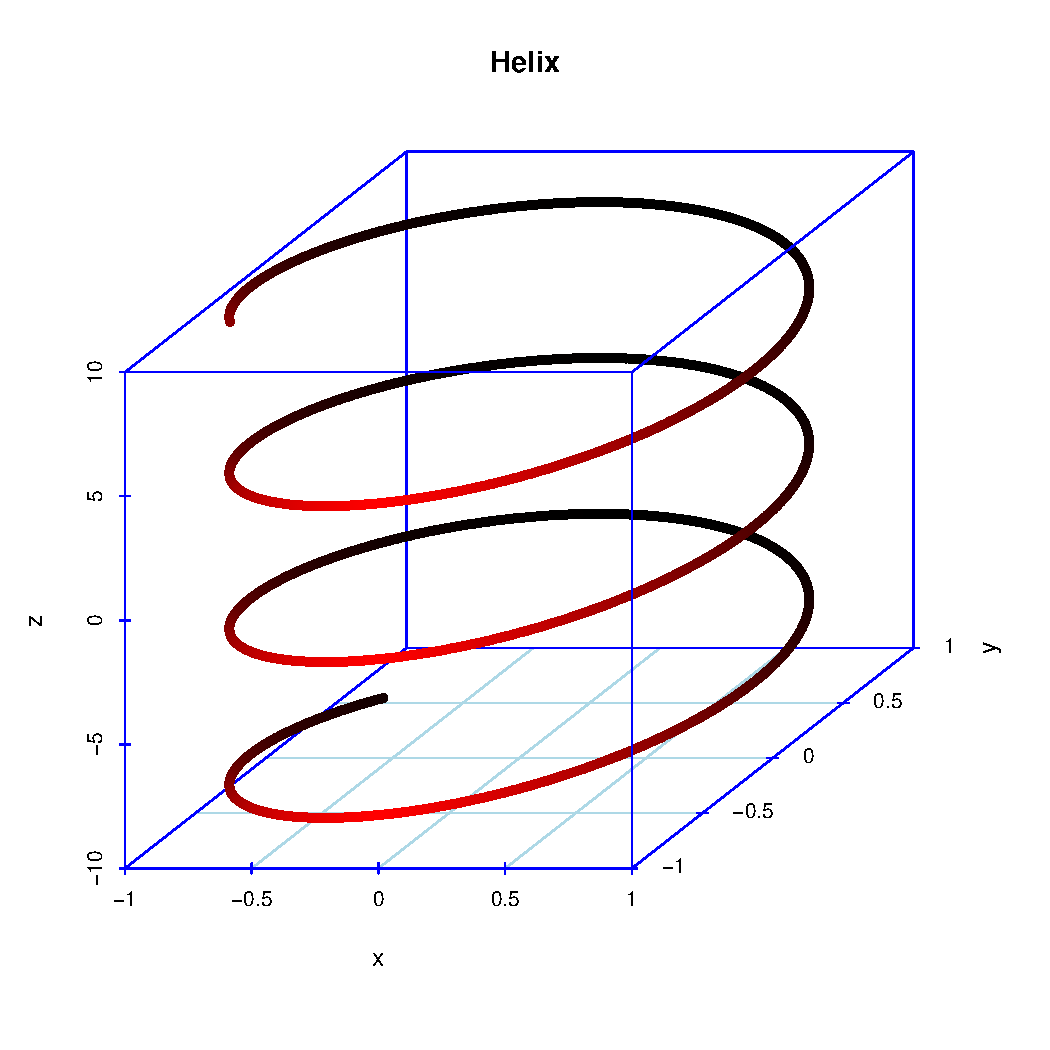
\includegraphics[width=13cm]{helix}
\end{center}
\vspace*{-10mm}\caption{Helix\label{helix}}
\end{figure}


\clearpage\subsubsection{Hemisphere}
Figure \ref{hemisphere} shows points on a hemisphere.
Except for  angle and the size of axes annotation, this figure is generated analogously to Figure \ref{helix}.

\vspace*{10mm}
\begin{figure}[htb!]
\small
\begin{Verbatim}[frame=single]
  temp <- seq(-pi, 0, length = 50)
  x <- c(rep(1, 50) %*% t(cos(temp)))
  y <- c(cos(temp)  %*% t(sin(temp)))
  z <- c(sin(temp)  %*% t(sin(temp)))
  scatterplot3d(x, y, z, highlight.3d = TRUE,  angle = 120,
           col.axis = "blue", col.grid = "lightblue", cex.axis = 1.3,
           cex.lab = 1.1, main = "Hemisphere", pch = 20)
\end{Verbatim}
\normalsize
\begin{center}
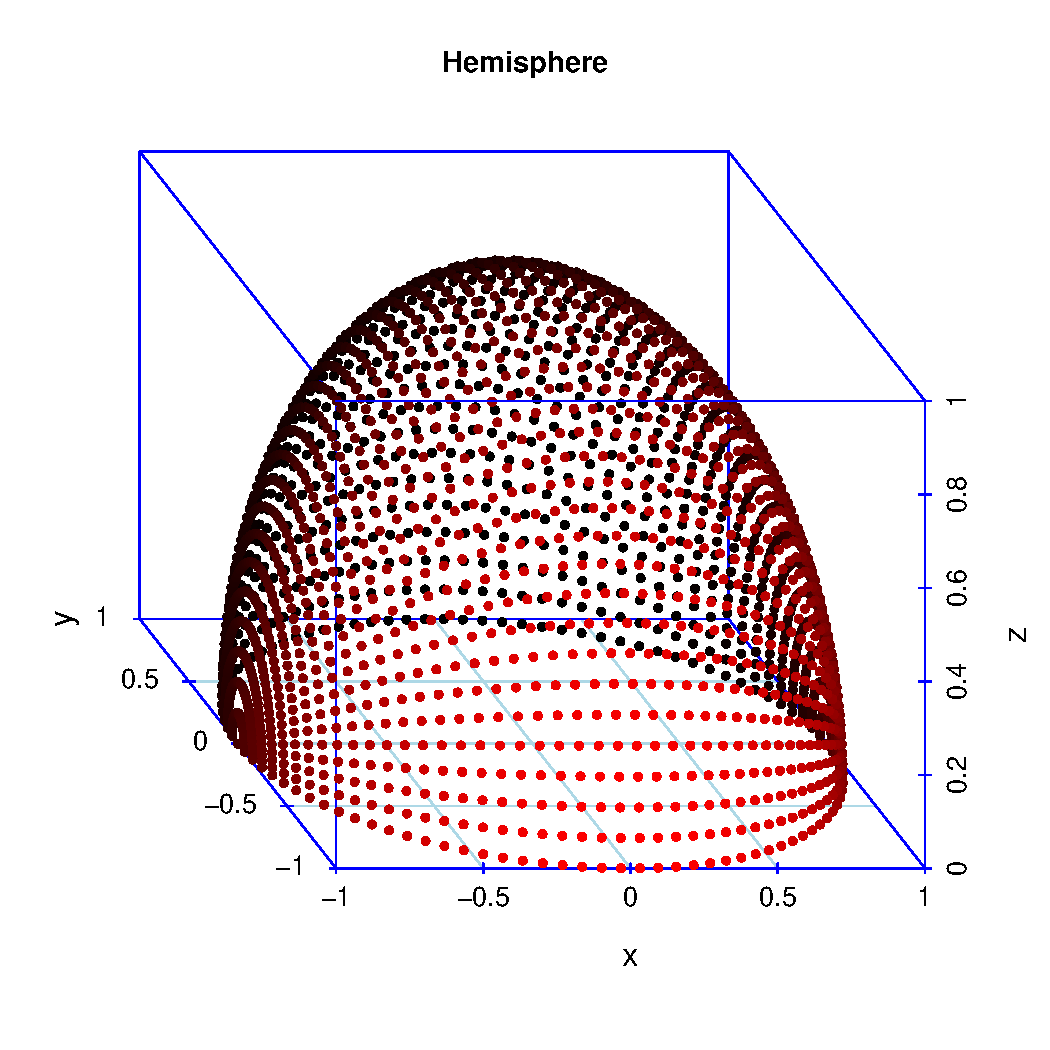
\includegraphics[width=13cm]{hemisphere}
\end{center}
\vspace*{-10mm}\caption{Hemisphere\label{hemisphere}}
\end{figure}


\clearpage\subsubsection{3D barplot}
With some simple modifications, it is possible to generate a 3D barplot, as shown in this example.
To make the plot look like a barplot, {\tt type = "h"} is set to draw vertical lines to the $x$--$y$ plane,
{\tt pch = " "} to avoid plotting of point symbols and {\tt lwd = 5} to make the lines looking like bars.
Furthermore, instead of three vectors a data frame is given as the first argument to \sdd .

\enlargethispage{1cm}
\vspace*{5mm}
\begin{figure}[htb!]
\small
\begin{Verbatim}[frame=single]
  my.mat <- matrix(runif(25), nrow = 5)
  dimnames(my.mat) <- list(LETTERS[1:5], letters[11:15])
  s3d.dat <- data.frame(columns = c(col(my.mat)),
                        rows    = c(row(my.mat)), value = c(my.mat))
  scatterplot3d(s3d.dat, type = "h", lwd = 5, pch = " ",
        x.ticklabs = colnames(my.mat), y.ticklabs = rownames(my.mat),
        color = grey(25:1 / 40), main = "3D barplot")
\end{Verbatim}
\normalsize
\begin{center}
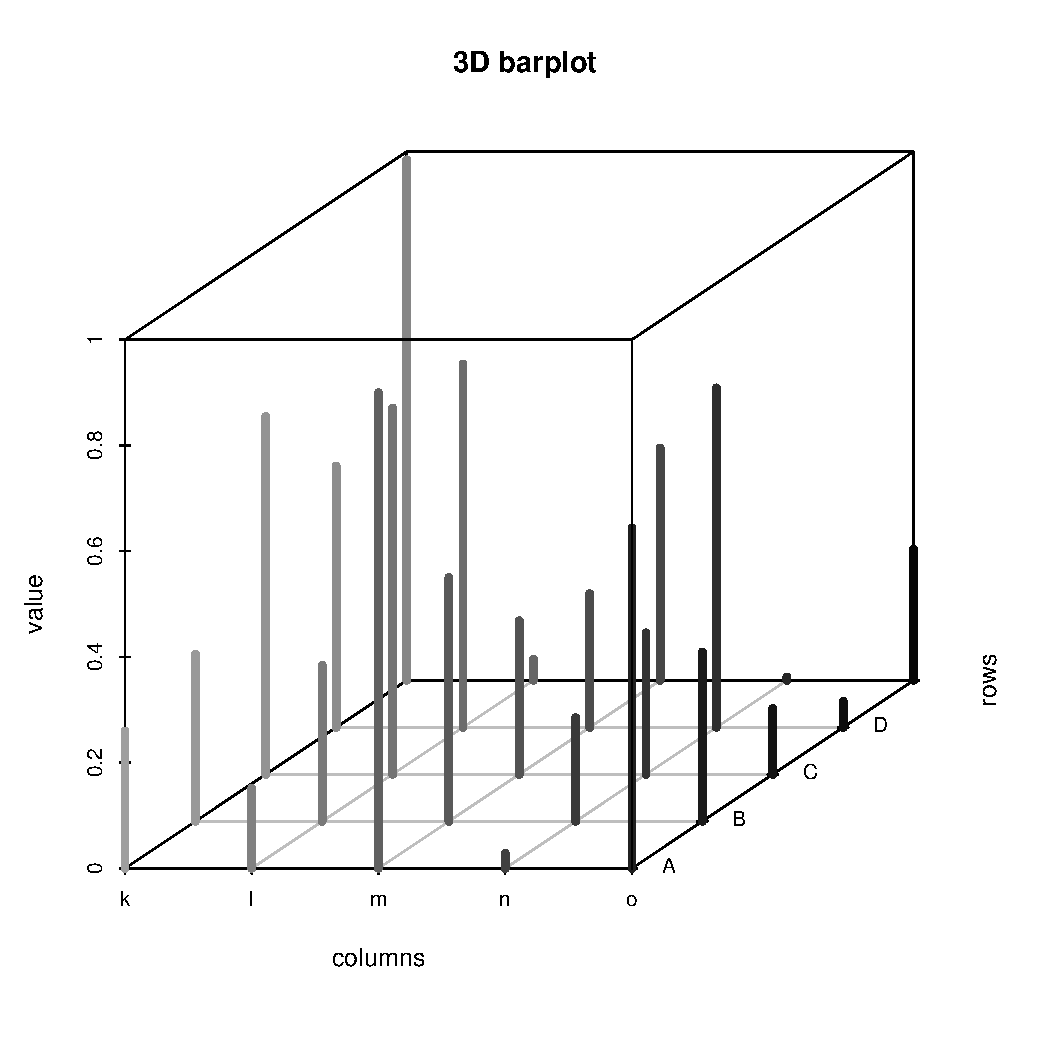
\includegraphics[width=12.5cm]{barplot}
\end{center}
\vspace*{-10mm}\caption{3D barplot\label{barplot}}
\end{figure}


\clearpage\subsubsection{Adding elements}
The importance of \textsl{Lexical Scoping} to generate \textsl{function closures}
to provide extensibility of \sdd\ was discussed in Section \ref{extend}.
An example how to use the invisibly returned functions is given below on the famous
(at least for \textsf{S} users) tree data.

After the tree data is loaded, it is plotted by \sdd ,
and the (invisibly returned) result is assigned to the variable {\tt s3d}.
The (blue colored) points are plotted using {\tt type = "h"},
so one can see the $x$--$y$ location of those points very clearly.

In the next step, a linear model (assumption: volume depends on girth and height of the trees) is calculated.
Furthermore, this \textsf{lm} object is plotted by the returned {\tt plane3d} function (was assigned to {\tt s3d} before),
and it results in a regression plane.

Just for demonstration purposes, in the last step some red colored points (on a imaginary line crossing the plot)
are plotted with an asterisk as its point symbol.

\vspace*{10mm}
\small
\begin{Verbatim}[frame=single]
  data(trees)
  s3d <- scatterplot3d(trees, type = "h", color = "blue",
      angle = 55, scale.y = 0.7, pch = 16, main = "Adding elements")
  my.lm <- lm(trees$Volume ~ trees$Girth + trees$Height)
  s3d$plane3d(my.lm)
  s3d$points3d(seq(10, 20, 2), seq(85, 60, -5), seq(60, 10, -10),
      col = "red", type = "h", pch = 8)
\end{Verbatim}
%$
\normalsize

\clearpage
\begin{figure}[htb!]
\begin{center}
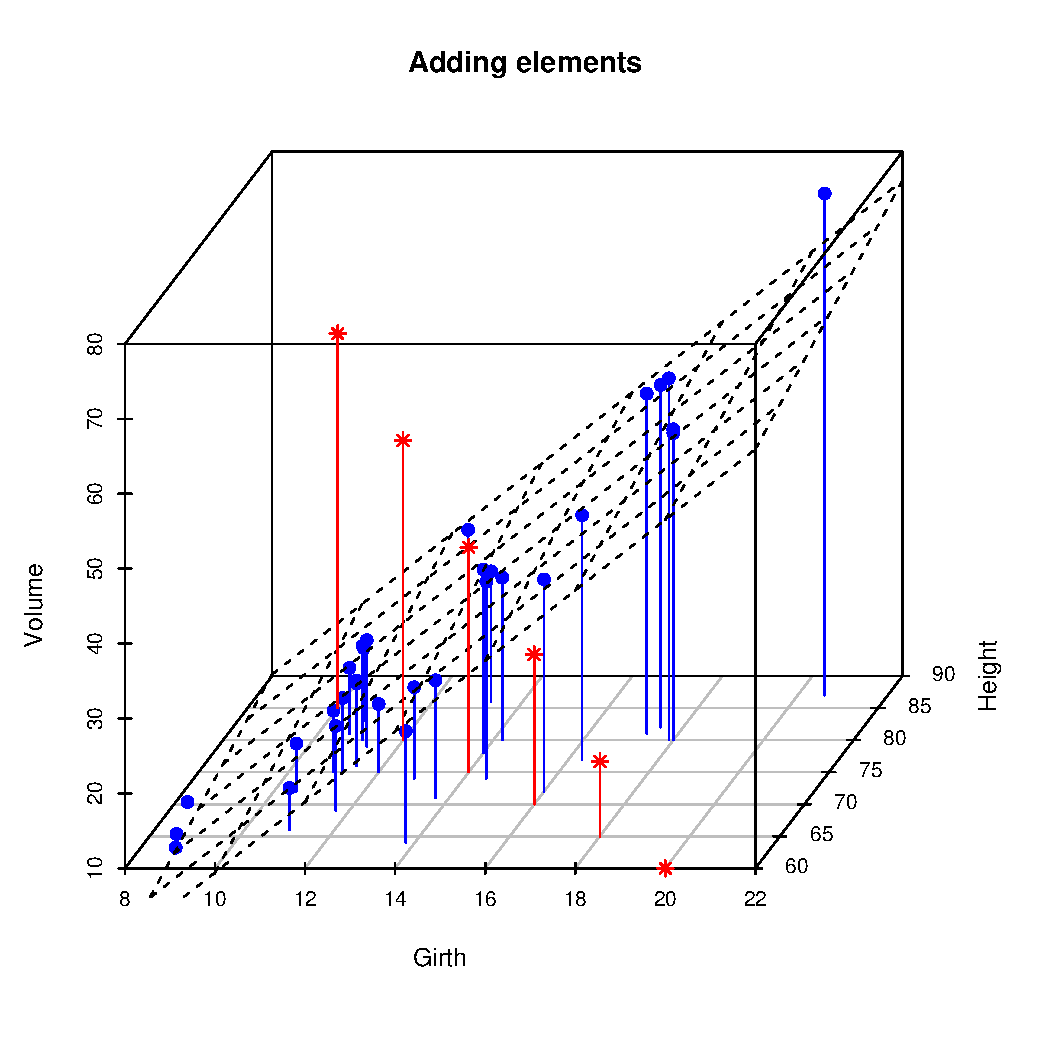
\includegraphics[width=13cm]{elements}
\end{center}
\vspace*{-10mm}\caption{Adding elements\label{elements}}
\end{figure}


\subsubsection{Bivariate normal distribution}
In Figure \ref{binorm} a surface of the density of a bivariate normal
distribution is plotted.  This example is a bit more sophisticated than the
examples before and shows the extensibility of \sdd.  Note that \sdd\
is designed to generate  scatter plots, not to draw surfaces,
is not really user friendly for this purpose, for which we'd typically
rather use \RR's \code{persp} function.

In a first step a matrix containing the density is calculated.
The call of \sdd\ sets up the plot (axes, labels, etc.), but doesn't draw
the surface itself which is accomplished by the two loops at the end of the
code.  Additionally, we give an example of quite sophisticated mathematical
annotation.
\clearpage
\small
\begin{Verbatim}[frame=single]
  library(mvtnorm)
  x1 <- x2 <- seq(-10, 10, length = 51)
  dens <- matrix(dmvnorm(expand.grid(x1, x2),
                    sigma = rbind(c(3, 2), c(2, 3))),
                 ncol = length(x1))
  s3d <- scatterplot3d(x1, x2,
                    seq(min(dens), max(dens), length = length(x1)),
                    type = "n", grid = FALSE, angle = 70,
                    zlab = expression(f(x[1], x[2])),
                    xlab = expression(x[1]), ylab = expression(x[2]),
                    main = "Bivariate normal distribution")
  text(s3d$xyz.convert(-1, 10, 0.07),
        labels = expression(f(x) == frac(1, sqrt((2 * pi)^n *
            phantom(".") * det(Sigma[X]))) * phantom(".") * exp{
            bgroup("(", - scriptstyle(frac(1, 2) * phantom(".")) *
                (x - mu)^T * Sigma[X]^-1 * (x - mu), ")")}))
  text(s3d$xyz.convert(1.5, 10, 0.05),
        labels = expression("with" * phantom("m") *
            mu == bgroup("(", atop(0, 0), ")") * phantom(".") * "," *
                phantom(0) *
            Sigma[X] ==  bgroup("(", atop(3 * phantom(0) * 2,
                2 * phantom(0) * 3), ")")))
  for(i in length(x1):1)
      s3d$points3d(rep(x1[i], length(x2)), x2, dens[i,], type = "l")
  for(i in length(x2):1)
      s3d$points3d(x1, rep(x2[i], length(x1)), dens[,i], type = "l")
\end{Verbatim}
\normalsize

\clearpage
\begin{figure}[htb!]
\begin{center}
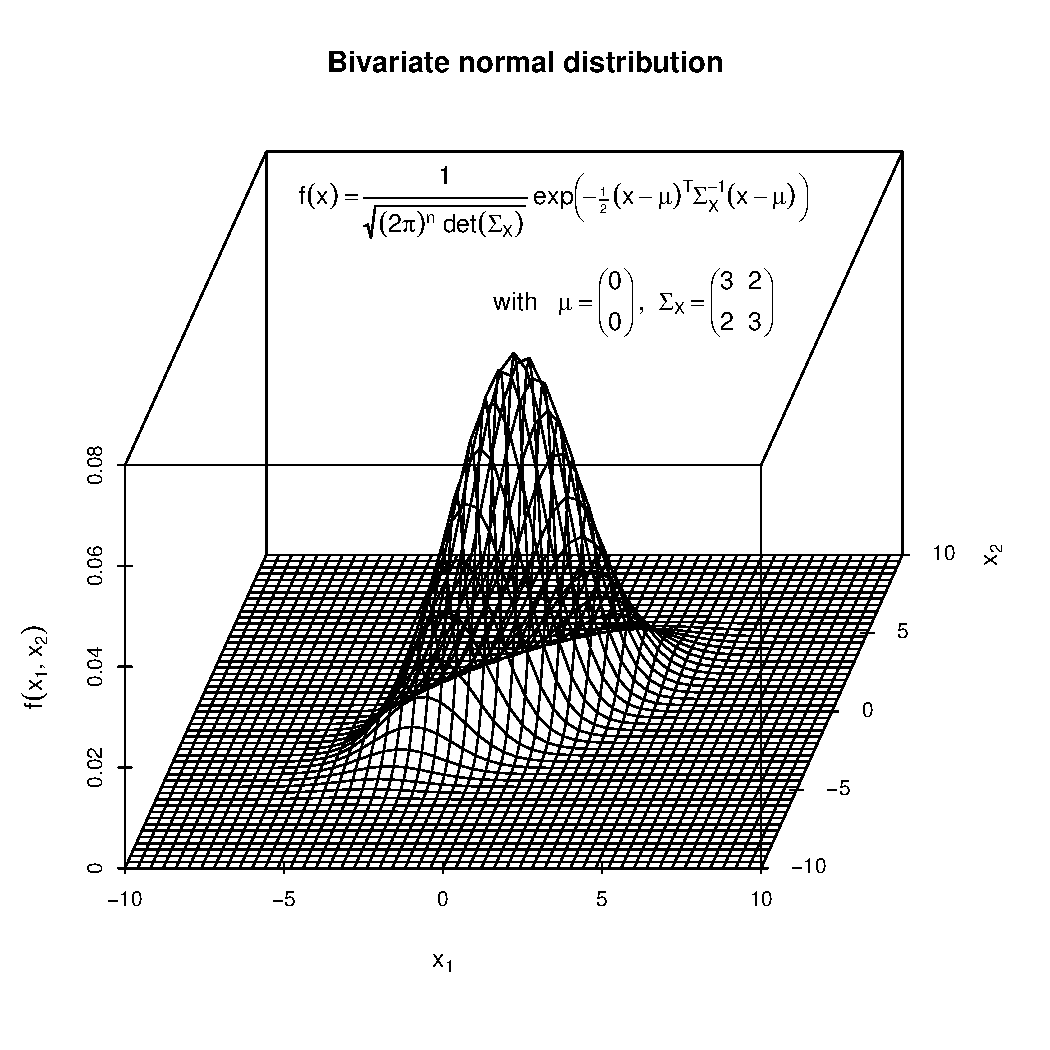
\includegraphics[width=13cm]{binorm}
\end{center}
\vspace*{-12mm}\caption{Density of a bivariate normal distribution\label{binorm}}
\end{figure}

\subsubsection{RGB color cube}
In Figure \ref{colorcube}, we visualize the RGB (red--green--blue) color
space which \RR{} and most computer screens use for color coding.
First, we draw all the \emph{named} colors available in \RR{} via
\texttt{colors()}.  Note that it might be interesting to find a better
background color here than white. Optimally it would correspond to an RGB
location as far away as possible from all given colors.
%%\enlargethispage{1cm}% Trick, damit es passt ...
Second, we show the \texttt{rainbow()} colors in the RGB space.  Here we
redraw the points \emph{on top} of the cube, using the \texttt{points3d()}
closure which is also the basis of our \texttt{cubedraw()} function.
\begin{figure}[htb!]
\small
%% to save space, suppressed things like
%%       ## Purpose: Draw nice cube with corners

%%   par(mfrow = 1:2)

\begin{Verbatim}[frame=single]
  cubedraw <- function(res3d, min = 0, max = 255, cex = 2)
  {
      cube01 <- rbind(0,c(1,0,0),c(1,1,0),1,c(0,1,1),c(0,0,1),c(1,0,1),
                        c(1,0,0),c(1,0,1),1,c(1,1,0),
                        c(0,1,0),c(0,1,1),  c(0,1,0),0)
      cub <- min + (max-min)* cube01
      res3d$points3d(cub[ 1:11,], cex = cex, type = 'b', lty = 1)
      res3d$points3d(cub[11:15,], cex = cex, type = 'b', lty = 3)
  }
  crgb <- t(col2rgb(cc <- colors()))
  rr <- scatterplot3d(crgb, color = cc, box = FALSE, angle = 24)
  cubedraw(rr)

  Rrb <- t(col2rgb(rbc <- rainbow(201)))
  rR <- scatterplot3d(Rrb, color = rbc, box = FALSE, angle = 24)
  cubedraw(rR)
  rR$points3d(Rrb, col = rbc, pch = 16)
\end{Verbatim}
\par\vspace*{-12mm}%$
\normalsize
\centerline{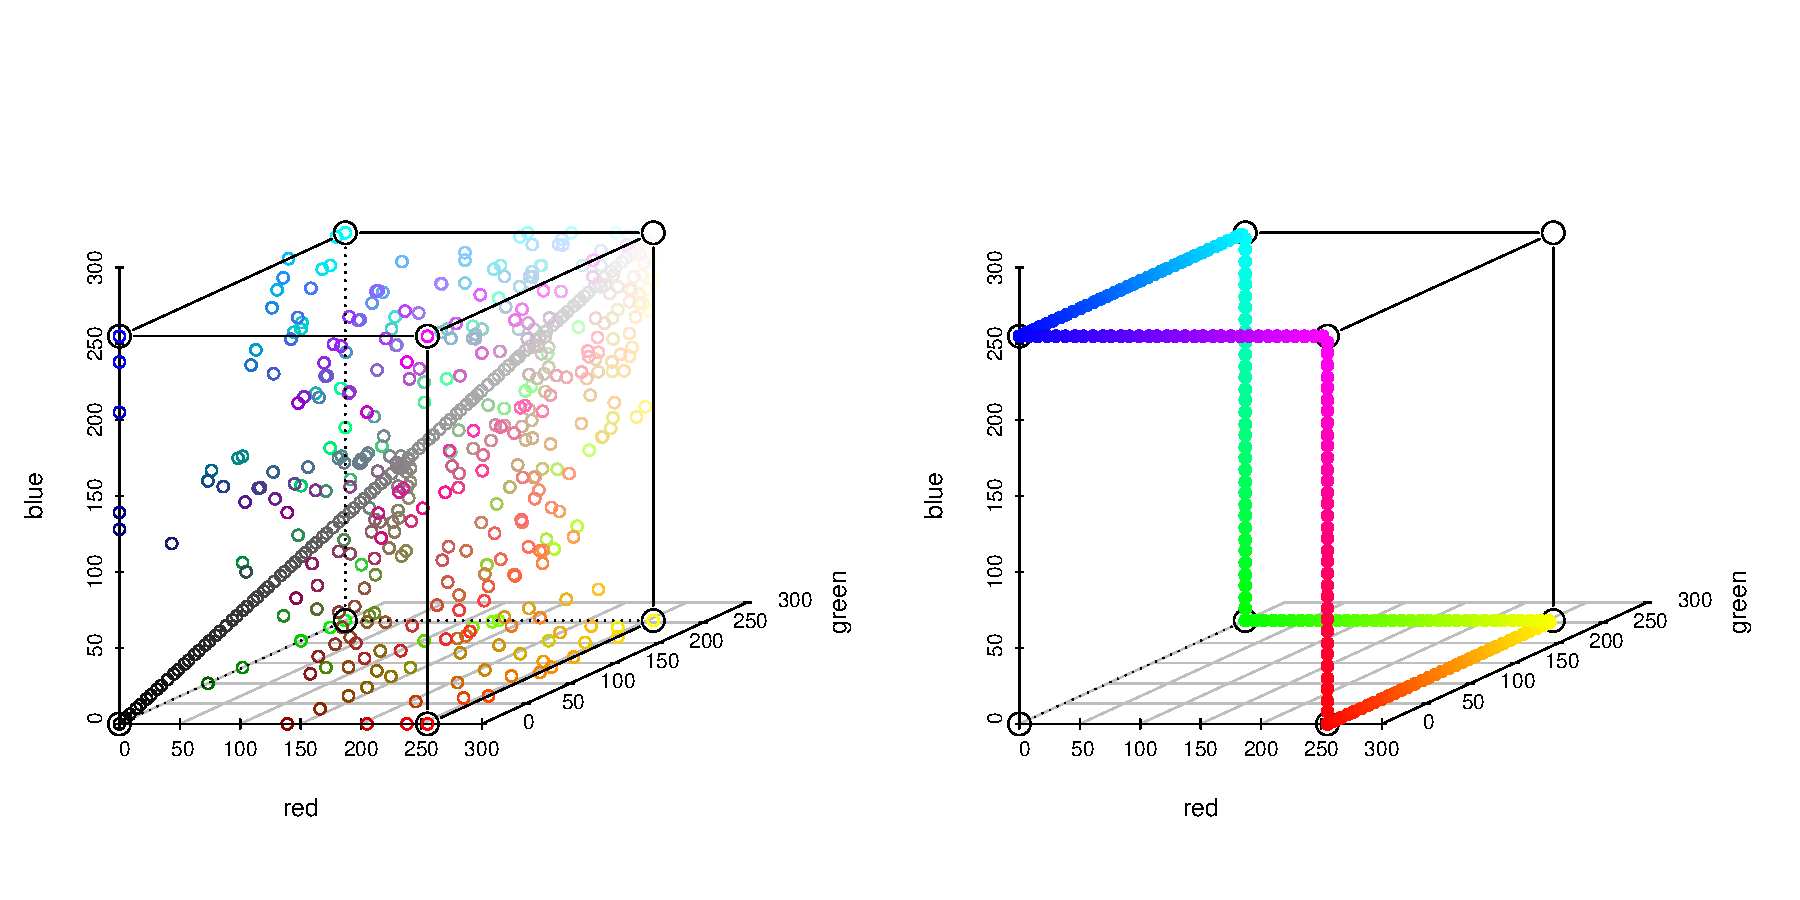
\includegraphics[width=19cm]{colorcube}}
\par\vspace*{-5mm}
\caption{The RGB color cube. On the left, the named colors in \RR{}, i.e.,
  \texttt{colors()}. Note the diagonal of gray tones. On the right, the
  locations and colors of \texttt{rainbow(201)}.\label{colorcube}}
\end{figure}





\clearpage
\subsection{Real world examples\label{realworld}}
Three real world examples are presented in this section.
The data are from the following recent projects of the collaborative
research centre 475
(Deutsche Forschungsgemeinschaft, SFB 475:
 ``Reduction of complexity in multivariate data structures''):

\vspace{-5mm}\begin{description}
\item[C3 \textmd{(Biometrics)}] Meta--Analysis in Biometry and Epidemiology,
\item[B3 \textmd{(Econometrics)}] Multivariate Analysis of Business Cycles, and
\item[C5 \textmd{(Technometrics)}]
    Analysis and Modelling of the Deephole--Drilling--Process with Methods of Statistics and Neuronal Networks.
\end{description}


\subsubsection{Meta--analysis of controlled clinical trials\label{meta}}
In the first real world example the data from a project on ``Meta--Analysis
in Biometry and Epidemiology'' is taken.
The data set contains the results of 13 placebo--controlled clinical trials
which evaluated the efficacy of the Bacillus Calmette--Gu\'{e}rin (BCG)
vaccine for the prevention of tuberculosis (TB).
%
An important task in combining the results of clinical trials is to detect
possible sources of heterogeneity which may influence the true treatment
effect.
%
In the present example, a possible influential covariate is the distance of
each trial from the equator, which may serve as a surrogate for the
presence of environmental mycobacteria that provide a certain level of
natural immunity against TB.
%
Other covariates may be the year the trial was carried out and the
allocation scheme of the vaccination
(A = alternate, R = random, S = systematic).
%%
For more details, especially on the choice of the trials and the
meta--analytical methods of combining the results, we refer to
\citeN{knapp02} and the references given therein.

In Figure \ref{fig:meta} the estimated risks of TB disease are plotted for the
vaccinated group and the non--vaccinated group, respectively, in the
dependence of the year the trial was carried out, of the absolute distance
from the equator and of the allocation scheme.
The color represents the precisions of the estimated risks.
Figure \ref{fig:meta} clearly reveals a spatio--temporal trend in the realization of the trials.
The former trials were carried out far away from the equator,
and in all these trials one can observe an evident superiority of the BCG vaccine for the prevention of TB.
Except one trial all the other later trials were realized closer to the equator.
In these trials, it is apparently that the estimated risks in the non--vaccinated groups are even rather low and,
consequently, cannot graphically separated from the estimated risks in the vaccinated groups.
Finally, it is worthwhile to note that the later trial which was carried out far away from the equator
has a relative small estimated risk in the non--vaccinated group compared to the former trials and, hence,
does not yield such an evident superiority of the BCG vaccine.

\begin{figure}[b!]
\small
\begin{Verbatim}[frame=single]
  layout(cbind(1:2, 1:2), heights = c(7, 1))
  prc <- hsv((prc <- 0.7 * Prec / diff(range(Prec))) - min(prc) + 0.3)
  s3d <- scatterplot3d(Year, Latitude, Risk, mar = c(5, 3, 4, 3),
      type = "h", pch = " ", main = "Estimated TB risks")
  s3d$points(Year, Latitude, Risk, pch = ifelse(vac, 22, 21), bg = prc,
      cex = ifelse(vac, 2, 1.5))
  s3d.coords <- s3d$xyz.convert(Year, Latitude, Risk)
  al.char <- toupper(substr(as.character(Allocation), 1, 1))
  text(s3d.coords$x[!vac], s3d.coords$y[!vac], labels = al.char[!vac],
      pos = 2, offset = 0.5)
  legend(s3d$xyz.convert(80, 15, 0.21), pch = c("A", "R", "S"), yjust=0,
      legend = c("alternate", "random", "systematic"), cex = 1.1)
  legend(s3d$xyz.convert(47, 60, 0.24), pch = 22:21, yjust = 0,
      legend = c("vaccinated", "not vaccinated"), cex = 1.1)

  par(mar=c(5, 3, 0, 3))
  plot(seq(min(Prec), max(Prec), length = 100), rep(0, 100), pch = 15,
      axes = FALSE, xlab = "color code of variable \"Precision\"",
      ylab = "", col = hsv(seq(0.3, 1, length = 100)))
  axis(1, at = 4:7, labels = expression(10^4, 10^5, 10^6, 10^7))
\end{Verbatim}
\end{figure}
\normalsize

Three variables are represented by the three dimensions of the cube, while
variable ``Precision'' is represented by color.  To realize color
representation for metric variables, some manual tuning is necessary,
though.

Two kinds of point symbols stand for the ``Vaccinated'' variable,
and for a sixth variable, ``Allocation'', an appropriate letter is printed
additionally close to the ``not vaccinated'' symbol.

For each of the latter three variables a legend is desirable.
Thus the smaller two legends are plotted into the \sdd ,
while the legend for the color coding gets a single plot.
The function {\tt layout} arranges the two plots suitably on the same device.

\begin{figure}[htb!]
\begin{center}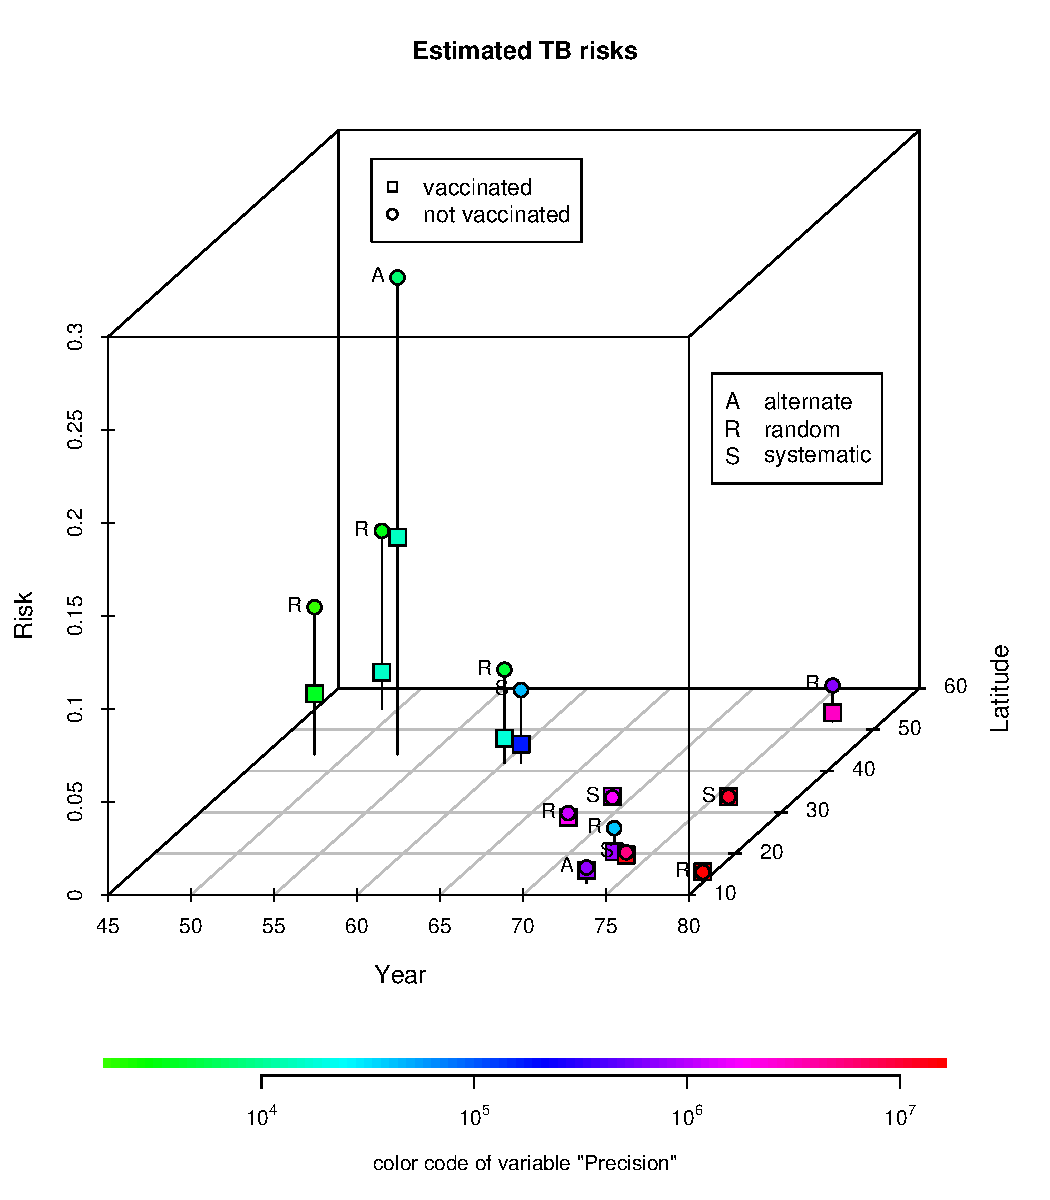
\includegraphics[width=13cm]{meta}\end{center}
\caption{Estimated TB risks\label{fig:meta}}
\end{figure}
\clearpage


\subsubsection{Business cycle data}
The example in this section shows the plotting of data from a project on ``Multivariate Analysis of Business Cycles''.
One of the main interests of the project is the prediction of business cycle phases.
An extraction of available relevant (concerning the purposes of this section) variables
and its abbreviations is given in Table \ref{StyFacts}.
The abbreviation 'gr' stands for growth rates with respect to last year's
corresponding quarter.

\begin{table}[htb!]
 \centering \vspace{0.2cm}
 \begin{tabular}{|l|l|}   \hline
 abbr & description                     \\ \hline
 IE & real investment in equipment (gr) \\
 C  & real private consumption (gr)     \\
 Y  & real gross national product (gr)  \\
 L  & wage and salary earners (gr)      \\ \hline
 \end{tabular}
 \caption{Abbreviations\label{StyFacts}}
\end{table}

The experts' classification of the data into business cycle phases
(``PH'') was done by \citeN{heilemann} using a 4-phase scheme.
These phases are called {\sl lower turning points}, {\sl upswing}, {\sl
  upper turning points}, and {\sl downswing}.

In Figure~\ref{business} the three variables C, Y, and L are represented by
the three dimensions of the cube.  The variable IE is represented by color,
while four different point symbols stand for the four business cycle phases
(PH).

For each of the latter two variables, a legend is desirable.
Thus the smaller one (for PH) is plotted into the \sdd , while the legend
for the color coding of IE got a single plot, analogously to the example in
Section~\ref{meta}.

A regression plane is added to the plot to support the visual impression.
Obviously all the plotted variables are highly correlated, with the
exception of the class variable which does not appear to be well
predictable by the other variables.  Details are discussed in
\citeN{theis99}.
%
In order to provide a correct impression of the fit, the residuals,
i.e. the projection lines to the plane, are drawn in Figure~\ref{residuals}
where different color and line types are used for positive and negative
residuals respectively.

\begin{figure}[H]
\vspace*{-10mm}
\footnotesize
\begin{Verbatim}[frame=single]
  layout(cbind(1:2, 1:2), heights = c(7, 1))
  temp <- hsv((temp <- 0.7 * IE / diff(range(IE))) - min(temp) + 0.3)
  s3d <- scatterplot3d(L, C, Y, pch = Phase, color = temp,
      mar = c(5, 3, 4, 3), main = "Business cycle phases")
  legend(s3d$xyz.convert(-2, 0, 16), pch = 1:4, yjust = 0,
      legend = c("upswing", "upper turning points",
          "downswing", "lower turning points"))
  s3d$plane3d(my.lm <- lm(Y ~ L + C), lty = "dotted")
  par(mar=c(5, 3, 0, 3))
  plot(seq(min(IE), max(IE), length = 100), rep(0, 100), pch = 15,
      axes = FALSE, xlab = "color code of variable \"IE\"", ylab = "",
      col = hsv(seq(0.3, 1, length = 100)))
  axis(1, at = seq(-20, 25, 5))
\end{Verbatim}
\normalsize
\begin{center}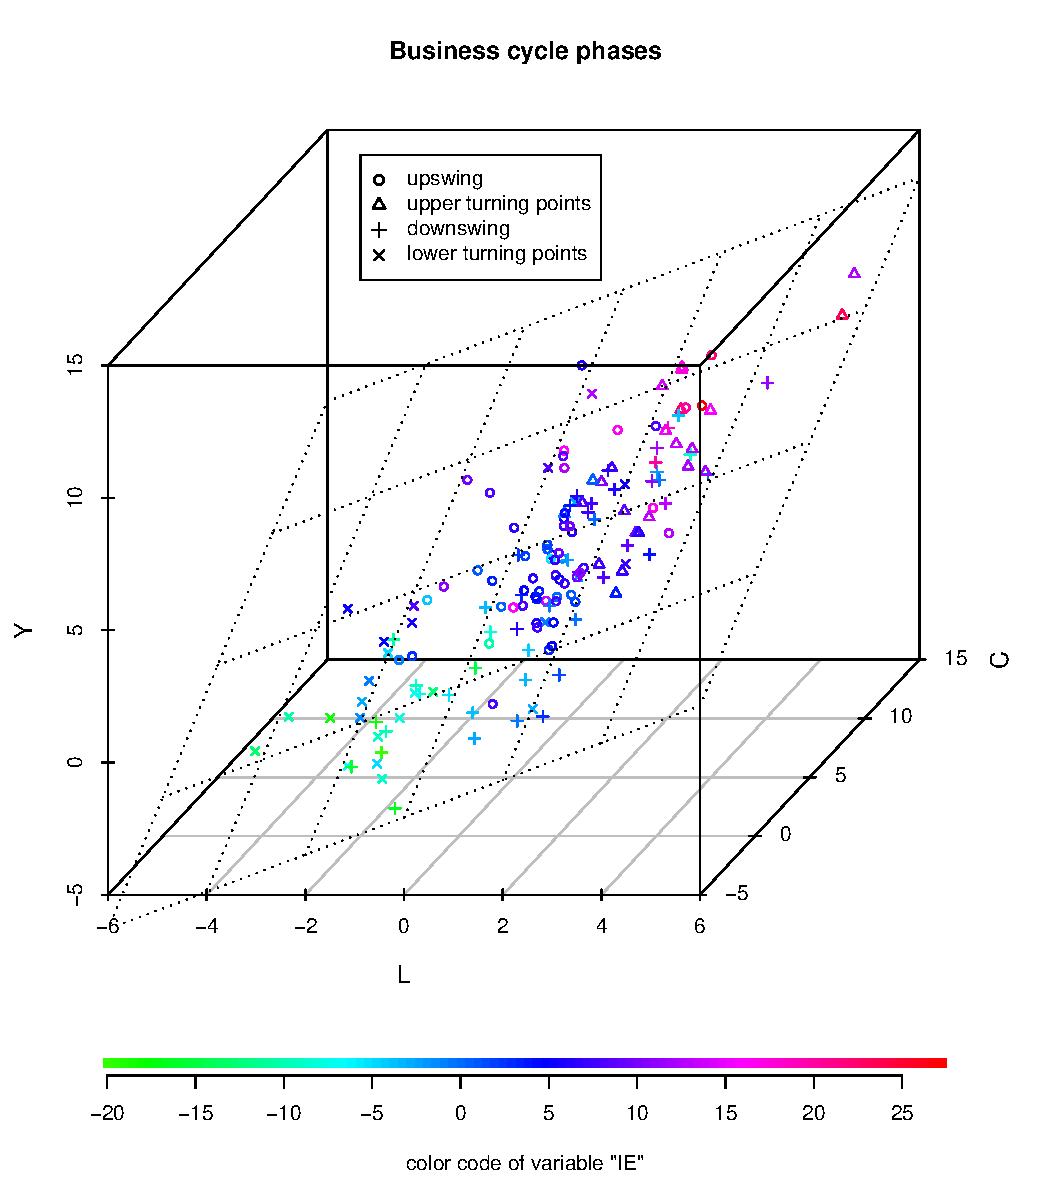
\includegraphics[width=13cm]{business}\end{center}
\vspace*{-5mm}\caption{Business cycle phases\label{business}}
\end{figure}

\begin{figure}[htb!]
\small
\begin{Verbatim}[frame=single]
  s3d <- scatterplot3d(L, C, Y, pch = 20, mar = c(5, 3, 4, 3),
            main = "Residuals")
  s3d$plane3d(my.lm, lty = "dotted")
  orig <- s3d$xyz.convert(L, C, Y)
  plane <- s3d$xyz.convert(L, C,  fitted(my.lm))
  i.negpos <- 1 + (resid(my.lm) > 0)
  segments(orig$x, orig$y, plane$x, plane$y,
            col = c("blue", "red")[i.negpos], lty = (2:1)[i.negpos])
\end{Verbatim}
%%$
\normalsize
\begin{center}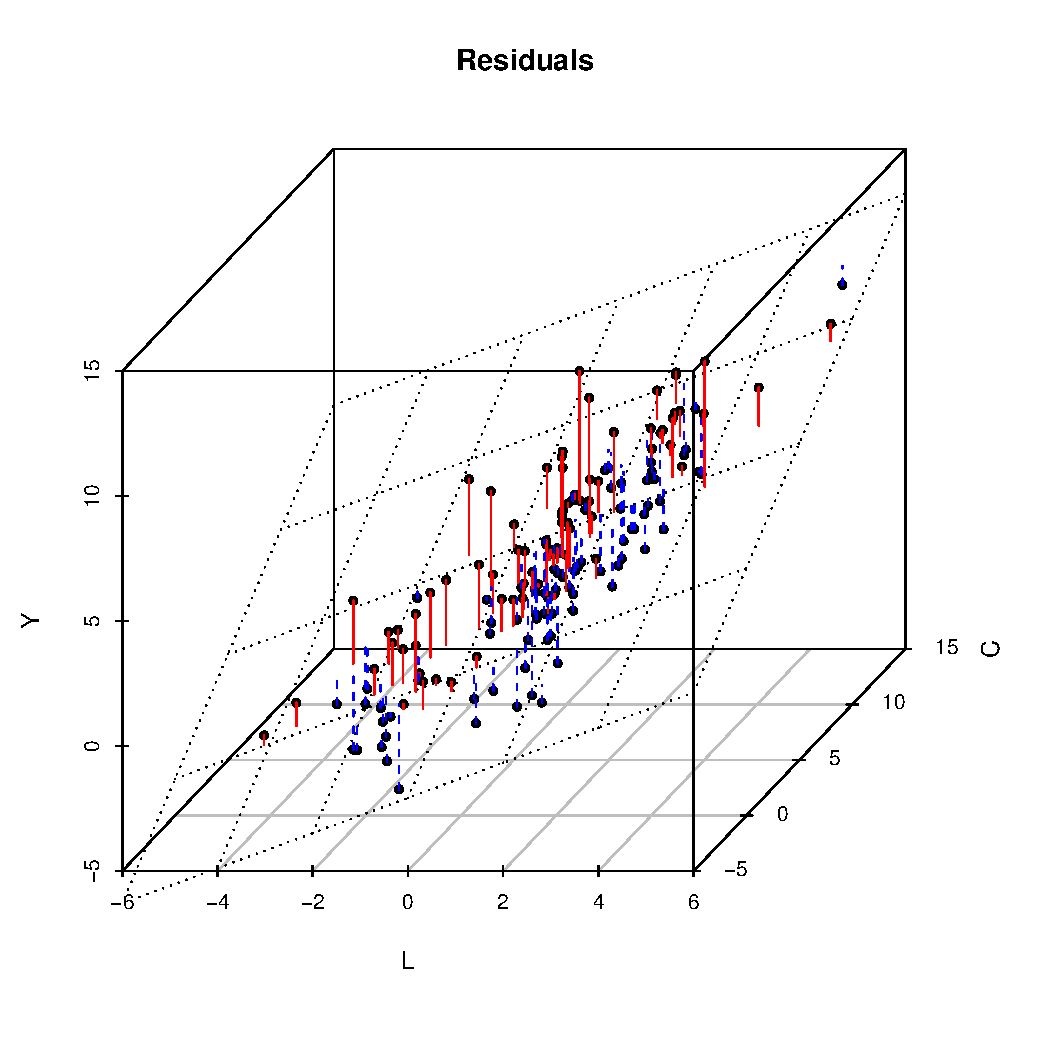
\includegraphics[width=13cm]{residuals}\end{center}
\vspace*{-5mm}\caption{Residuals (cf. Figure \ref{business})\label{residuals}}
\end{figure}


\clearpage
\subsubsection{Deep hole drilling}
Our last real world example shows phase spaces (\cite{tong93}) of the drilling torque of a deep hole drilling process.
The data is taken from a project on
"Analysis and Modelling of the Deephole--Drilling--Process with Methods of Statistics and Neuronal Networks".
More detailed analysis on the data than provided in the following example was done by,
e.g., \citeN{busse} and \citeN{weinert}.

Figure \ref{drill1} visualizes the phase spaces of the drilling torques of two deep hole drilling processes,
a regular and a chattering one.
Obviously the points in the phase space of the chattering process are very systematically scattered,
and the range of the data is very different for the two processes.
The magnification of the regular process in Figure \ref{drill2} shows that the points of the regular process are scattered
unsystematically.
Note that other lags like 10, 20, 100 would produce a similar plot.
This indicates a sine wave like relationship in the chattering case.

\vspace{10mm}
\small
\begin{Verbatim}[frame=single]
  s3d <- scatterplot3d(drill1[1:400], drill1[7:406], drill1[32:431],
      color = "red", type = "l", angle = 120, xlab = "drilling torque",
      ylab = "drilling torque, lag 6", zlab = "drilling torque, lag 31",
      main = "Two deep hole drilling processes")
  s3d$points3d(drill2[1:400], drill2[7:406], drill2[32:431],
      col = "blue", type = "l")
  legend(s3d$xyz.convert(-400, 1000, 950), col= c("blue", "red"),
      legend = c("regular process", "chattering process"), lwd = 2,
      bg = "white")

  scatterplot3d(drill2[1:400], drill2[7:406], drill2[32:431],
      color = "blue", type = "l", angle = 120, xlab = "drilling torque",
      ylab = "drilling torque, lag 6", zlab = "drilling torque, lag 31",
      main = "Magnification of the regular process")
\end{Verbatim}
\normalsize

\begin{figure}[htb!]
\vspace*{-15mm}
\begin{center}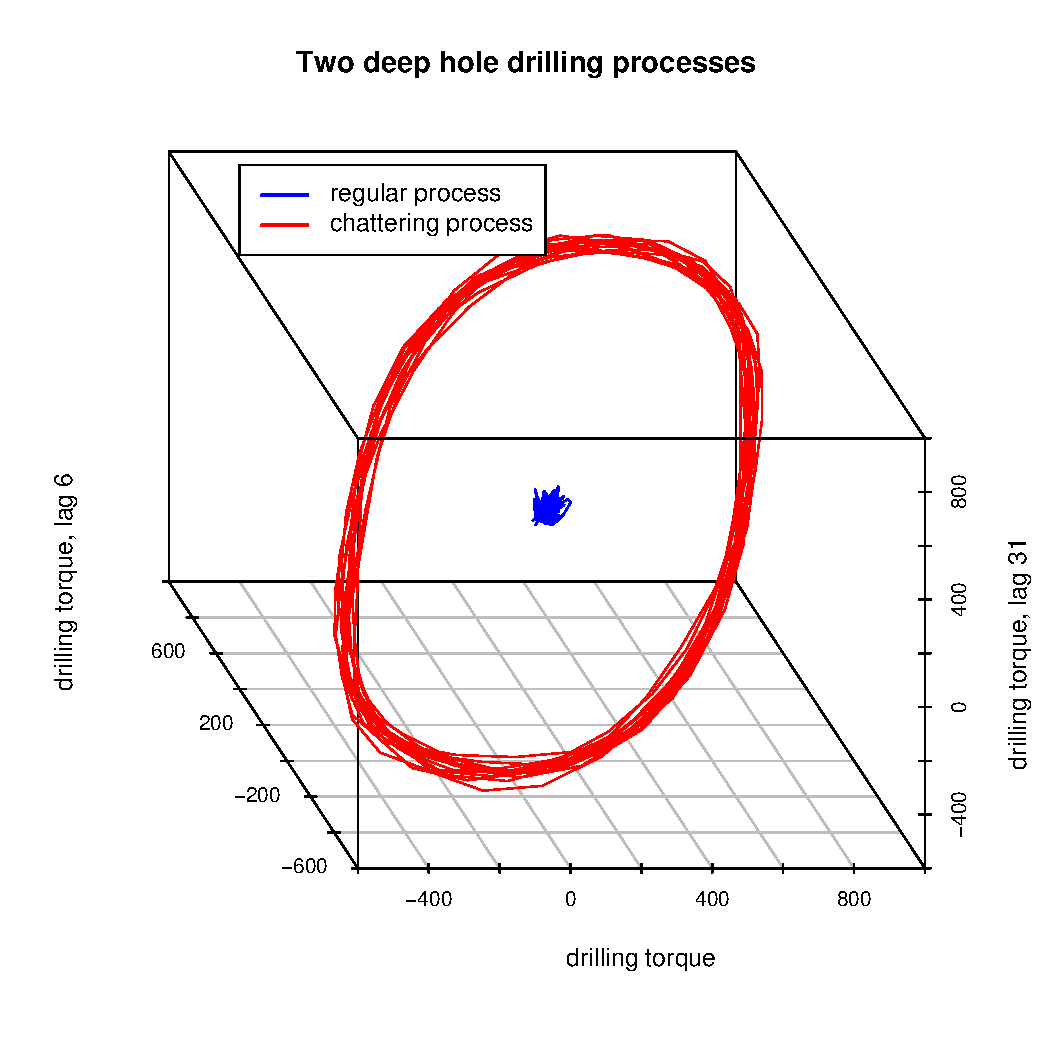
\includegraphics[width=11.5cm]{drill1}
\vspace*{-10mm}\caption{Phase spaces of the drilling torques of two deep hole drilling processes\label{drill1}}
\vspace*{10mm}
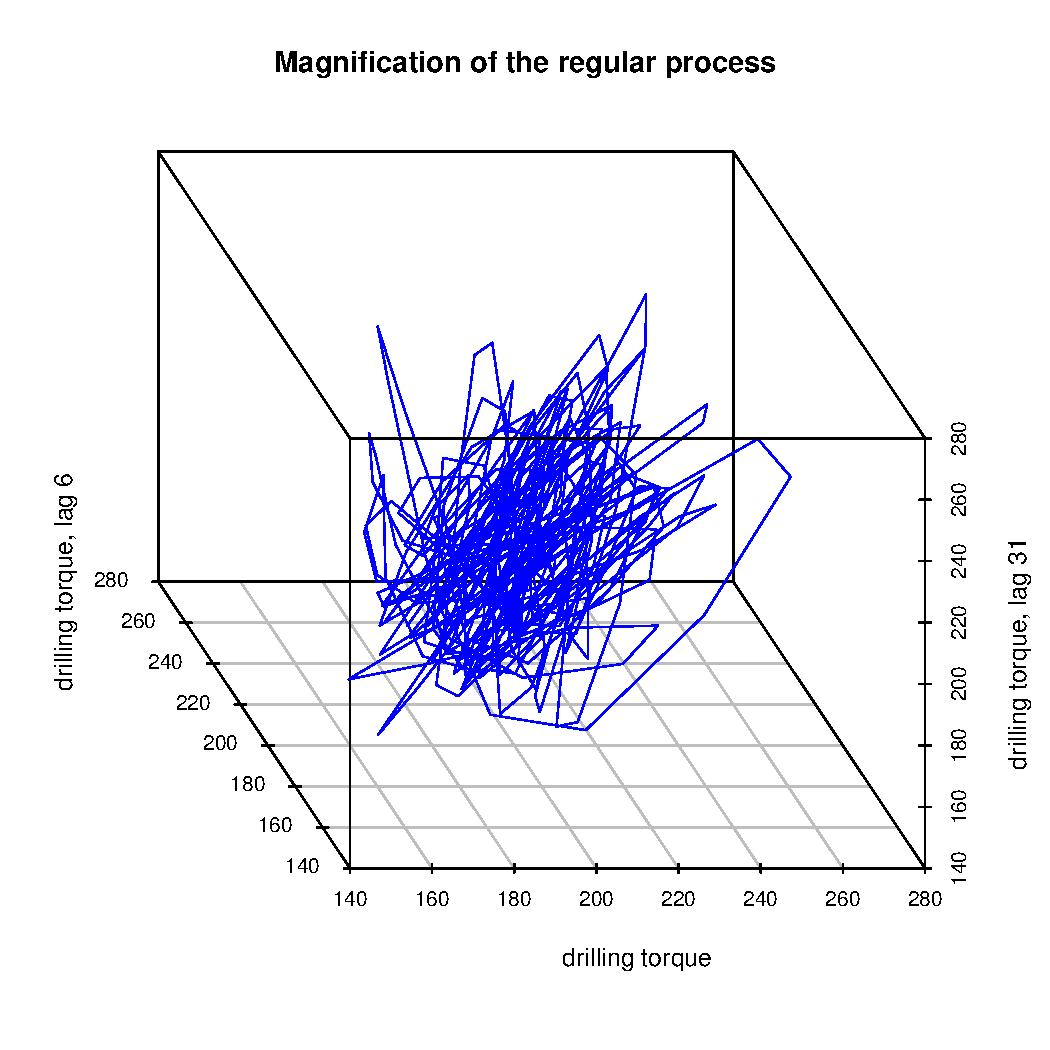
\includegraphics[width=11.5cm]{drill2}\end{center}
\vspace*{-10mm}\caption{Magnification of the regular process (Figure \ref{drill1})\label{drill2}}
\end{figure}
\clearpage

\section{Other 3D tools in \RR\label{tools}}
At the time of writing \sdd , the function \code{persp()} in the base
package of \RR\ for three dimensional surface plots was available, but
there was no way to generate 3D scatter plots in \RR\ itself.

The data visualization system \emph{xgobi} (\cite{swayne98}) provides
interactive visualization of multidimensional data, e.g. brush and spin,
higher-dimensional rotation, grand tour, etc.  The \RR\ package
\emph{xgobi} (\cite{swayne91}; we have to distinguish the visualization
system and the package) provides an Interface to \emph{xgobi} and launches
a \emph{xgobi} process appropriately.
%%
\emph{ggobi}\footnote{\url{http://www.ggobi.org}}
(\cite{swayne02}) is the next edition of \emph{xgobi}.

Analogously to \emph{xgobi} a \RR\ package \emph{Rggobi} (\cite{temple01})
exists in the \emph{Omegahat} project\footnote{\url{http://www.omegahat.net}}
(\cite{temple00}) that allows one to embed \emph{ggobi} within
\RR\ and to both set and query the \emph{ggobi} contents.  All in all,
\emph{ggobi} can be loaded dynamically into \RR\ (as well as into other
software products, in principle), and \RR\ into \emph{ggobi}.  This
provides interactive, direct manipulation, linked, high-dimensional
graphics within \RR .

The package \emph{rgl}\footnote{\url{http://wsopuppenkiste.wiso.uni-goettingen.de/~dadler/rgl/}}
by \cite{AdlerNenadic2003} is a portable \RR\ programing interface to \emph{OpenGL}.
Its features include, e.g., interactive viewpoint navigation,
automatic data focus, up to 8 light sources, alpha-blending
(transparency), and environmental effects like fogging.
The package \emph{djmrgl}\footnote{This package was
formerly called \emph{rgl}, similar to the other mentioned package
by Daniel Adler and Oleg Nenadi\'{c}.
\emph{djmrgl} is only available for the Windows operating system.}
(\cite{murdoch}) also provides an \RR\ interface to \emph{OpenGL}.
A huge collection of useful functions to generate,
manipulate and interactively rotate 3D objects is available.
Efforts are under way to merge these two packages.

The function \code{cloud} in the lattice package is a 3D scatter plot function that works in the
\emph{lattice} (\cite{sarkar02}) (and \emph{grid} (\cite{murrell01}))
environment of \RR .
\emph{Lattice} is an implementation of \emph{Trellis Graphics}, which is a
framework for data visualization developed at the Bell Labs by
\citeN{becker96}, extending ideas presented in \citeN{cleveland}.


\section{Conclusion\label{conclusion}}
In the design (Section \ref{design}) of the scatter plot function \sdd\ emphasis is placed on generality and extensibility
(Section \ref{extend}).
These two properties are demonstrated in Section \ref{examples}, as well as the high printout quality.
A high printout quality and a homogeneous appearance with respect of any other \RR\ (2D) graphics is extremely important
for publications and presentations. Thus we recommend to use \sdd\ particularly for these purposes.

Other \RR\ related 3D ``tools'' (Section \ref{tools}) are focused on different properties,
such as surface plotting (e.g. function {\tt persp}), interactivity and online analysis (e.g. \emph{ggobi} or \emph{RGL}).


\section*{Acknowledgements}
The financial support of the Deutsche Forschungsgemeinschaft
(SFB 475, ``Reduction of complexity in multivariate data structures") is gratefully acknowledged.

We express our sincere thanks to the following people (in alphabetical order)
for their extensive comments on the features and bugs during the time of development,
as well as for the discussion of the example data:\\
Ben Bolker, Anja Busse, Ursula Garczarek, Joachim Hartung, Guido Knapp, Winfried Theis, Brigitta Vo\ss, and Claus Weihs.




\bibliographystyle{chicago}
\bibliography{ligges}
\clearpage
\begin{appendix}
\section*{Appendix -- help page}
\small
\HeaderA{scatterplot3d}{3D Scatter Plot}{scatterplot3d}
\keyword{hplot}{scatterplot3d}
\begin{Description}\relax
Plots a three dimensional (3D) point cloud.
\end{Description}
\begin{Usage}
\begin{verbatim}
scatterplot3d(x, y=NULL, z=NULL, color=par("col"), pch=NULL,
    main=NULL, sub=NULL, xlim=NULL, ylim=NULL, zlim=NULL,
    xlab=NULL, ylab=NULL, zlab=NULL, scale.y=1, angle=40,
    axis=TRUE, tick.marks=TRUE, label.tick.marks=TRUE,
    x.ticklabs=NULL, y.ticklabs=NULL, z.ticklabs=NULL,
    y.margin.add=0, grid=TRUE, box=TRUE, lab=par("lab"),
    lab.z=mean(lab[1:2]), type=par("type"), highlight.3d=FALSE,
    mar=c(5,3,4,3)+0.1, col.axis=par("col.axis"),
    col.grid="grey", col.lab=par("col.lab"),
    cex.symbols=par("cex"), cex.axis=par("cex.axis"),
    cex.lab=0.8 * par("cex.lab"), font.axis=par("font.axis"),
    font.lab=par("font.lab"), lty.axis=par("lty"),
    lty.grid=par("lty"), lty.hide=NULL, log="", ...)
\end{verbatim}
\end{Usage}
\begin{Arguments}
\begin{ldescription}
\item[\code{x}] the coordinates of points in the plot.
\item[\code{y}] the y coordinates of points in the plot, optional if \code{x} is an appropriate structure.
\item[\code{z}] the z coordinates of points in the plot, optional if \code{x} is an appropriate structure.
\item[\code{color}] colors of points in the plot, optional if \code{x} is an appropriate structure.
Will be ignored if \code{highlight.3d = TRUE}.
\item[\code{pch}] plotting "character", i.e. symbol to use.
\item[\code{main}] an overall title for the plot.
\item[\code{sub}] sub-title.
\item[\code{xlim, ylim, zlim}] the x, y and z limits (min, max) of the plot. Note that setting enlarged limits
may not work as exactly as expected (a known but unfixed bug).
\item[\code{xlab, ylab, zlab}] titles for the x, y and z axis.
\item[\code{scale.y}] scale of y axis related to x- and z axis.
\item[\code{angle}] angle between x and y axis (Attention: result depends on
scaling.  For 180 < angle < 360  the returned functions
\code{xyz.convert} and \code{points3d} will not work properly.).
\item[\code{axis}] a logical value indicating whether axes should be drawn on the plot.
\item[\code{tick.marks}] a logical value indicating whether tick marks should
be drawn on the plot (only if \code{axis = TRUE}).
\item[\code{label.tick.marks}] a logical value indicating whether tick marks should be labeled on the plot
(only if \code{axis = TRUE} and \code{tick.marks = TRUE}).
\item[\code{x.ticklabs, y.ticklabs, z.ticklabs}] vector of tick mark labels.
\item[\code{y.margin.add}] add additional space between tick mark labels and
axis label of the y axis
\item[\code{grid}] a logical value indicating whether a grid should be drawn on the plot.
\item[\code{box}] a logical value indicating whether a box should be drawn around the plot.
\item[\code{lab}] a numerical vector of the form c(x, y, len).  The values of
x and y give the (approximate) number of tickmarks on the x and y axes.
\item[\code{lab.z}] the same as \code{lab}, but for z axis.
\item[\code{type}] character indicating the type of plot: "p" for points, "l"
for lines, "h" for vertical lines to x-y-plane, etc.
\item[\code{highlight.3d}] points will be drawn in different colors related to y coordinates
(only if \code{type = "p"} or \code{type = "h"}, else \code{color} will be used).\\
On some devices not all colors can be displayed. In this case try the
postscript device or use \code{highlight.3d = FALSE}.
\item[\code{mar}] A numerical vector of the form c(bottom, left, top, right)
which gives the lines of margin to be specified on the four sides of the plot.
\item[\code{col.axis, col.grid, col.lab}] the color to be used for axis / grid / axis labels.
\item[\code{cex.symbols, cex.axis, cex.lab}] the magnification to be used for
point symbols, axis annotation, labels relative to the current.
\item[\code{font.axis, font.lab}] the font to be used for axis annotation / labels.
\item[\code{lty.axis, lty.grid}] the line type to be used for axis / grid.
\item[\code{lty.hide}] line style used to plot \sQuote{non-visible} edges (defaults of the \code{lty.axis} style)
\item[\code{log}] Not yet implemented!  A character string which contains "x"
(if the x axis is to be logarithmic), "y", "z", "xy", "xz", "yz", "xyz".
\item[\code{...}] more graphical parameters can be given as arguments,
\code{pch = 16} or \code{pch = 20} may be nice.
\end{ldescription}
\end{Arguments}
\begin{Value}
\begin{ldescription}
\item[\code{xyz.convert}] function which converts coordinates from 3D (x, y, z)
to 2D-projection (x, y) of \code{scatterplot3d}.
Useful to plot objects into existing plot.
\item[\code{points3d}] function which draws points or lines into the existing plot.
\item[\code{plane3d}] function which draws a plane into the existing plot:
\code{plane3d(Intercept, x.coef = NULL, y.coef = NULL, lty =
      "dashed", lty.box = NULL, ...)}.
Instead of \code{Intercept} a vector containing 3
elements or an (g)lm object can be specified.
The argument \code{lty.box} allows to set a different line style for the
intersecting lines in the box's walls.
\item[\code{box3d}] function which "refreshes" the box surrounding the plot.
\end{ldescription}
\end{Value}
\begin{Note}\relax
Some graphical parameters should only be set as arguments in
\code{scatterplot3d} but not in a previous \code{\LinkA{par}{par}()} call.  One of these is
\code{mar}, which is also non-standard in another way: Users who
want to extend an existing \code{scatterplot3d} graphic with another function than
\code{points3d}, \code{plane3d} or \code{box3d}, should consider to
set \code{par(mar = c(b, l, t, r))} to the value of \code{mar} used in
\code{scatterplot3d}, which defaults to \code{c(5, 3, 4, 3) + 0.1}.

Other \code{par} arguments may be split into several arguments in
\code{scatterplot3d}, e.g., for specifying the line type.  And finally
some of \code{par} arguments do not apply here, e.g., many of those
for axis calculation.  So we recommend to try the specification of
graphical parameters at first as arguments in \code{scatterplot3d} and
only if needed as arguments in previous \code{par()} call.
\end{Note}
\begin{Author}\relax
Uwe Ligges \email{ligges@statistik.tu-dortmund.de};
\url{http://www.statistik.tu-dortmund.de/~ligges}.
\end{Author}
\begin{References}\relax
Ligges, U., and Maechler, M. (2003):
Scatterplot3d -- an R Package for Visualizing Multivariate Data.
\emph{Journal of Statistical Software} 8(11), 1--20.
\url{http://www.jstatsoft.org/}
\end{References}
\begin{SeeAlso}\relax
\code{\LinkA{persp}{persp}}, \code{\LinkA{plot}{plot}}, \code{\LinkA{par}{par}}.
\end{SeeAlso}
\begin{Examples}
\begin{ExampleCode}
  ## On some devices not all colors can be displayed.
  ## Try the postscript device or use highlight.3d = FALSE.
  ## example 1
  z <- seq(-10, 10, 0.01)
  x <- cos(z)
  y <- sin(z)
  scatterplot3d(x, y, z, highlight.3d=TRUE, col.axis="blue",
      col.grid="lightblue", main="scatterplot3d - 1", pch=20)

  ## example 2
  temp <- seq(-pi, 0, length = 50)
  x <- c(rep(1, 50) %*% t(cos(temp)))
  y <- c(cos(temp) %*% t(sin(temp)))
  z <- c(sin(temp) %*% t(sin(temp)))
  scatterplot3d(x, y, z, highlight.3d=TRUE,
      col.axis="blue", col.grid="lightblue",
      main="scatterplot3d - 2", pch=20)

  ## example 3
  temp <- seq(-pi, 0, length = 50)
  x <- c(rep(1, 50) %*% t(cos(temp)))
  y <- c(cos(temp) %*% t(sin(temp)))
  z <- 10 * c(sin(temp) %*% t(sin(temp)))
  color <- rep("green", length(x))
  temp <- seq(-10, 10, 0.01)
  x <- c(x, cos(temp))
  y <- c(y, sin(temp))
  z <- c(z, temp)
  color <- c(color, rep("red", length(temp)))
  scatterplot3d(x, y, z, color, pch=20, zlim=c(-2, 10),
      main="scatterplot3d - 3")

  ## example 4
  my.mat <- matrix(runif(25), nrow=5)
  dimnames(my.mat) <- list(LETTERS[1:5], letters[11:15])
  my.mat # the matrix we want to plot ...

  s3d.dat <- data.frame(cols=as.vector(col(my.mat)),
      rows=as.vector(row(my.mat)),
      value=as.vector(my.mat))
  scatterplot3d(s3d.dat, type="h", lwd=5, pch=" ",
      x.ticklabs=colnames(my.mat), y.ticklabs=rownames(my.mat),
      color=grey(25:1/40), main="scatterplot3d - 4")

  ## example 5
  data(trees)
  s3d <- scatterplot3d(trees, type="h", highlight.3d=TRUE,
      angle=55, scale.y=0.7, pch=16, main="scatterplot3d - 5")
  # Now adding some points to the "scatterplot3d"
  s3d$points3d(seq(10,20,2), seq(85,60,-5), seq(60,10,-10),
      col="blue", type="h", pch=16)
  # Now adding a regression plane to the "scatterplot3d"
  attach(trees)
  my.lm <- lm(Volume ~ Girth + Height)
  s3d$plane3d(my.lm, lty.box = "solid")

  ## example 6; by Martin Maechler
  cubedraw <- function(res3d, min = 0, max = 255, cex = 2,
    text. = FALSE)
  {
    ## Purpose: Draw nice cube with corners
    cube01 <- rbind(c(0,0,1), 0, c(1,0,0),
                    c(1,1,0), 1, c(0,1,1), # < 6 outer
                    c(1,0,1), c(0,1,0))
                        # <- "inner": fore- & back-ground
    cub <- min + (max-min)* cube01
    ## visibile corners + lines:
    res3d$points3d(cub[c(1:6,1,7,3,7,5) ,],
        cex = cex, type = 'b', lty = 1)
    ## hidden corner + lines
    res3d$points3d(cub[c(2,8,4,8,6),     ],
        cex = cex, type = 'b', lty = 3)
    if(text.)## debug
        text(res3d$xyz.convert(cub), labels=1:nrow(cub),
            col='tomato', cex=2)
  }
  ## 6 a) The named colors in R, i.e. colors()
  cc <- colors()
  crgb <- t(col2rgb(cc))
  par(xpd = TRUE)
  rr <- scatterplot3d(crgb, color = cc, box = FALSE, angle = 24,
      xlim = c(-50, 300), ylim = c(-50, 300), zlim = c(-50, 300))
  cubedraw(rr)
  ## 6 b) The rainbow colors from rainbow(201)
  rbc <- rainbow(201)
  Rrb <- t(col2rgb(rbc))
  rR <- scatterplot3d(Rrb, color = rbc, box = FALSE, angle = 24,
      xlim = c(-50, 300), ylim = c(-50, 300), zlim = c(-50, 300))
  cubedraw(rR)
  rR$points3d(Rrb, col = rbc, pch = 16)
\end{ExampleCode}
\end{Examples}


\end{appendix}
\end{document}
